\section{Current Progress}
Currently, the progress related to each topic is listed below:
\begin{itemize}

\item \textbf{Active Learning}
 \begin{itemize}
  \item Gained a general understanding of the theory
  \item Diving into applications of different sampling framework in pratical problem
  \item Primary framework programming and testing 
 \end{itemize}
 
 
 For the learning process, I employed the SVM and Bayesian frame- work. And for querying strategy, I used Random Sampling, uncertainty Sampling. The test dataset is used is the Digit11, the dataset used in The Semi-Supervised Learning Book. This dataset includes 1500 instances and each one has 241 features. Below is the result of the current program- ming.
 \begin{figure}[htbp]
  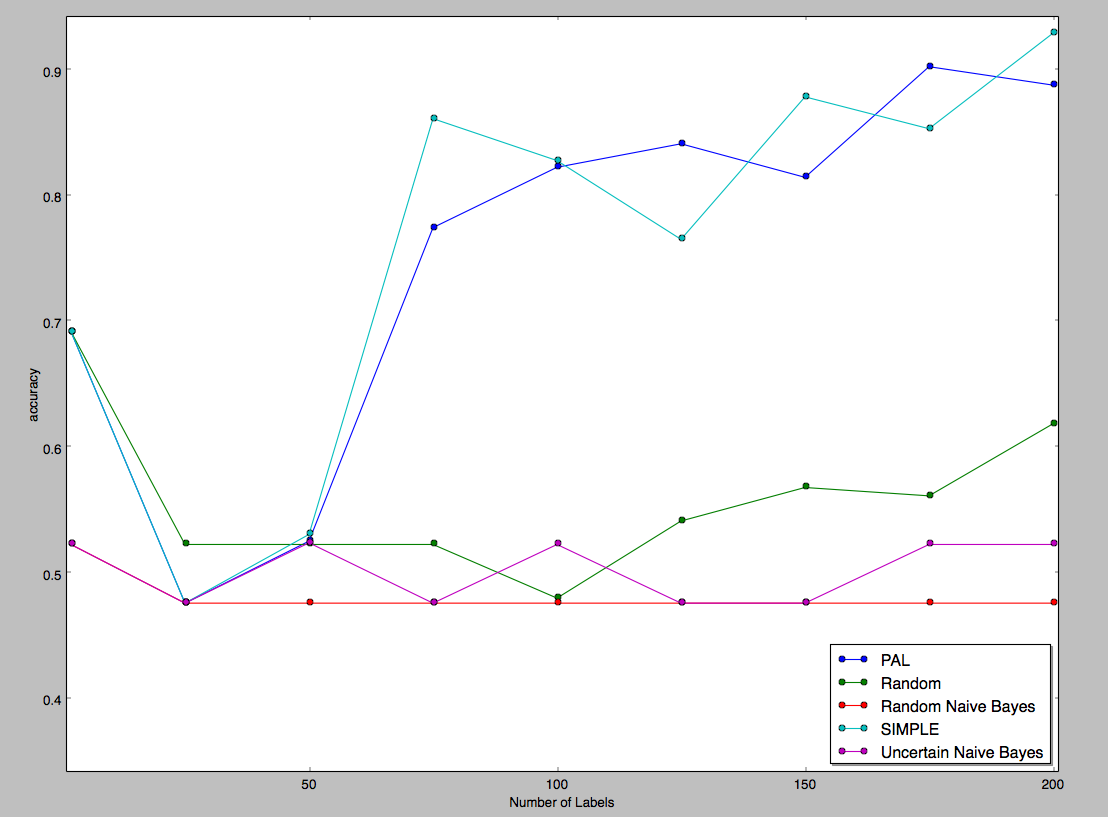
\includegraphics[scale=0.3]{activelearning/report}
  \caption{Active learning result}
 \end{figure}

As can be seen from the figure, if active sampling procedure is applied, the performance is on average better than random sampling method(the base test of the test). 


\item \textbf{Bayesian Nonparametric Model}
 \begin{itemize}
  \item Gained a general understanding of the theory
  \item Currently reviewing on the Gaussian process used for BNP regression
  \item Primary framework programming 
 \end{itemize}
 \end{itemize}